\section{QR-Zerlegung}
\begin{frame}
	\frametitle{QR-Zerlegung}
	\vspace{-4cm}
	\begin{itemize}
		\item $ A = QR $
	\end{itemize}
\end{frame}

\begin{frame}
	\frametitle{Householder-Transformation}
	\vspace{-1cm}
	\begin{align*}
		H = I - 2 \dfrac{vv^T}{v^Tv}
	\end{align*}
	\centering
	\scalebox{.8}{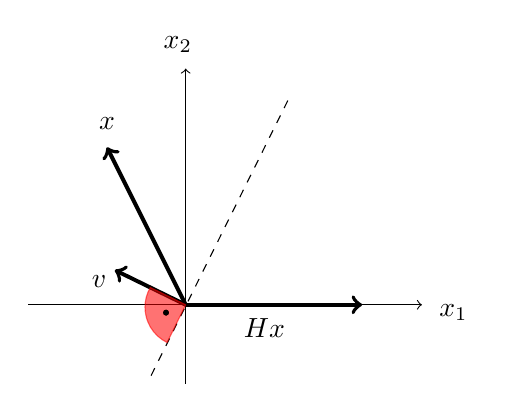
\begin{tikzpicture}
\filldraw[red, opacity=0.1] (0,0)--(-0.45, 0.22) arc (150:244:.5cm) -- (0,0) ;
\filldraw(-0.25,-0.1) circle (.03cm) ;

\draw[->] (-2,0) -- (3,0);
\draw[->] (0,-1) -- (0,3);

\draw[->,line width=0.5mm] (0,0) -- (-1,2);
\draw[->,line width=0.5mm] (0,0) -- (2.24,0);

\draw[dashed] (-0.44,-0.9) -- (1.34,2.68);
\draw[->,line width=0.5mm] (0,0) -- (-0.9, 0.44);


\draw (3.4,-0.1) node {$x_1$};
\draw (-0.1,3.3) node {$x_2$};

\filldraw[red, opacity=0.5] (0,0)--(-0.45, 0.22) arc (150:244:.5cm) -- (0,0) ;
\filldraw(-0.25,-0.1) circle (.03cm) ;

\draw (-1.1, 0.3) node {$v$};
\draw (-1, 2.3) node {$x$};
\draw (1,-0.3) node {$Hx$};


\end{tikzpicture}}

\end{frame}

\begin{frame}
	\frametitle{Householder-Transformation}
	\vspace{-1cm}
	\begin{itemize}
	\item Householder Vektor berechnen\\
		\begin{itemize}
			\item Ansatz $ Hx = \alpha e_1 $
			\item Normieren $ v_1 = 1 $
			\item $ \tau = \dfrac{2}{v^Tv} \quad \Longrightarrow \quad H = I - 2 \dfrac{vv^T}{v^Tv} = I - \tau vv^T$
		\end{itemize}
		
%		$\alpha = -1 \cdot \text{sign}(x_1) \|x\|_2$\\
%		$\tau = \dfrac{\alpha - x_1}{\alpha}$\\
%		$v=\dfrac{x - \alpha e_1}{x_1 - \alpha}$ 

	\item  Householder-Transformation anwenden
		\begin{align*} 
		H A =(I - \tau vv^T) A= A - \tau (vv^T )A = A - \tau v(v^TA)
		\end{align*}
	\end{itemize}
\end{frame}

\begin{frame}
	\frametitle{QR-Zerlegung mittels Householder}

	\begin{itemize}
		\item $ A = QR $
		\only<1>{
		\begin{align*}
			H_1 A &= \left( 
			\begin{array}{cccc}
			* & * & * & * \\ 
			0 & * & * & * \\ 
			0 & * & * & * \\ 
			0 & * & * & *
			\end{array}
			\right)
		\end{align*} 
		}
		\only<2>{
		\begin{align*}
			H_2 H_1 A &= \left( 
			\begin{array}{cccc}
			* & * & * & * \\ 
			0 & * & * & * \\ 
			0 & 0 & * & * \\ 
			0 & 0 & * & *
			\end{array}
			\right)
		\end{align*} 
		}
	\only<3>{
		\begin{align*}
		H_3 H_2 H_1 A &= \left( 
		\begin{array}{cccc}
		* & * & * & * \\ 
		0 & * & * & * \\ 
		0 & 0 & * & * \\ 
		0 & 0 & 0 & *
		\end{array}
		\right)
		\end{align*} 
	}
	\only<4>{
		\begin{align*}
		H_3 H_2 H_1 A &= \left( 
		\begin{array}{cccc}
		r_{1,1} & r_{1,2}  & r_{1,3}  & r_{1,4}  \\ 
		v_2^{(1)} & r_{2,2} & r_{2,3}  & r_{2,4}  \\ 
		v_3^{(1)} & v_3^{(2)} & r_{3,3}  & r_{3,4}  \\ 
		v_4^{(1)} & v_4^{(2)} & v_4^{(3)} & r_{4,4} 
		\end{array}
		\right)
		\end{align*} 
	}
	\item
	\begin{align*}
	H_1 = \begin{pmatrix}
	\hat{H_1} 
	\end{pmatrix} \qquad , \qquad
	H_2 = \left(\begin{array}{l|l}
	I_{1} & 0\\ \hline
	0 & \hat{H_2} 	
	\end{array} \right)\qquad , \qquad
	H_i = \left(\begin{array}{l|l}
	I_{i-1} & 0\\ \hline
	0 & \hat{H_i} 	
	\end{array} \right)
	\end{align*}
	\end{itemize}
\end{frame}

\begin{frame}
	\frametitle{Benchmark}
	\begin{itemize}
		\item Rechner
		\item Peak performance
		\item Flops
		\item Aufwand QR Householder
	\end{itemize}
\end{frame}

\begin{frame}
	\frametitle{Ungeblockte QR}
	\centering
	\scalebox{.85}{
		\includegraphics[width=\textwidth]{images/unblk}
	}
\end{frame}

\begin{frame}
	\frametitle{Geblockte QR-Zerlegung}
	\begin{itemize}
		\item Matrix A\\
		\centering
		\clearpage
\setcounter{page}{8}
\begin{frame}
\frametitle{Geblockte QR-Zerlegung}
\begin{itemize}
	\item Matrix A\\
	\centering
	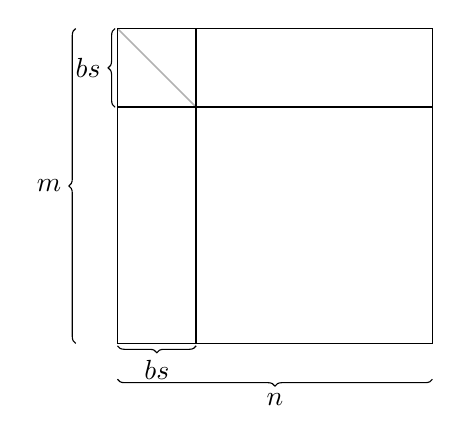
\begin{tikzpicture}
	\draw[semithick] (0,0) -- (4,0) -- (4,4) -- (0,4) -- (0,0);
	
		\draw[semithick] (1,0) -- (1,4);
		\draw[semithick] (0,3) -- (4,3);
		\draw[semithick,opacity=0.3] (0,4) -- (1,3);
		\draw[decorate, decoration={brace,mirror}, yshift=-.2ex]  (0,0) -- node[below=0.4ex] {$bs$}  (1,0);
		\draw[decorate, decoration={brace}, xshift=-.2ex]  (0,3) -- node[left=0.4ex] {$bs$}  (0,4);
	
		%\draw (0.5,3.5) node {$A_{0,0}$};
		%\draw (0.5,1.5) node {$A_{bs,0}$};
		%\draw (2.5,3.5) node {$A_{0,bs}$};
		%\draw (2.5,1.5) node {$A_{bs,bs}$};
		%\draw[decorate, decoration={brace,mirror}, yshift=-.2ex]  (0,0) -- node[below=0.4ex] {$bs$}  (1,0);
		%\draw[decorate, decoration={brace}, xshift=-.2ex]  (0,3) -- node[left=0.4ex] {$bs$}  (0,4);
		\draw[decorate, decoration={brace,mirror}, yshift=-3ex]  (0,0) -- node[below=0.4ex] {$n$}  (4,0);
		\draw[decorate, decoration={brace}, xshift=-3.5ex]  (0,0) -- node[left=0.4ex] {$m$}  (0,4);
	\end{tikzpicture}
\end{itemize}
\end{frame}

\clearpage
\setcounter{page}{8}
\begin{frame}
\frametitle{Geblockte QR-Zerlegung}
\begin{itemize}
	\item Matrix A\\
	\centering
	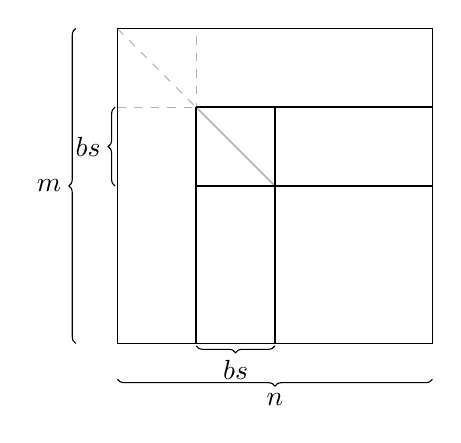
\begin{tikzpicture}
	\draw[semithick] (0,0) -- (4,0) -- (4,4) -- (0,4) -- (0,0);
	

		\draw[dashed,opacity=0.3] (1,0) -- (1,4);
		\draw[dashed,opacity=0.3] (0,3) -- (4,3);
		\draw[dashed,opacity=0.3] (0,4) -- (1,3);
		\draw[semithick] (2,0) -- (2,3);
		\draw[semithick] (1,2) -- (4,2);
		\draw[semithick] (1,0) -- (1,3);
		\draw[semithick] (1,3) -- (4,3);
		\draw[semithick,opacity=0.3] (1,3) -- (2,2);
		\draw[decorate, decoration={brace,mirror}, yshift=-.2ex]  (1,0) -- node[below=0.4ex] {$bs$}  (2,0);
		\draw[decorate, decoration={brace}, xshift=-.2ex]  (0,2) -- node[left=0.4ex] {$bs$}  (0,3);
	
	

	
	%\draw (0.5,3.5) node {$A_{0,0}$};
	%\draw (0.5,1.5) node {$A_{bs,0}$};
	%\draw (2.5,3.5) node {$A_{0,bs}$};
	%\draw (2.5,1.5) node {$A_{bs,bs}$};
	%\draw[decorate, decoration={brace,mirror}, yshift=-.2ex]  (0,0) -- node[below=0.4ex] {$bs$}  (1,0);
	%\draw[decorate, decoration={brace}, xshift=-.2ex]  (0,3) -- node[left=0.4ex] {$bs$}  (0,4);
	\draw[decorate, decoration={brace,mirror}, yshift=-3ex]  (0,0) -- node[below=0.4ex] {$n$}  (4,0);
	\draw[decorate, decoration={brace}, xshift=-3.5ex]  (0,0) -- node[left=0.4ex] {$m$}  (0,4);
	
	\end{tikzpicture}
\end{itemize}
\end{frame}

\clearpage
\setcounter{page}{8}
\begin{frame}
\frametitle{Geblockte QR-Zerlegung}
\begin{itemize}
	\item Matrix A\\
	\centering
	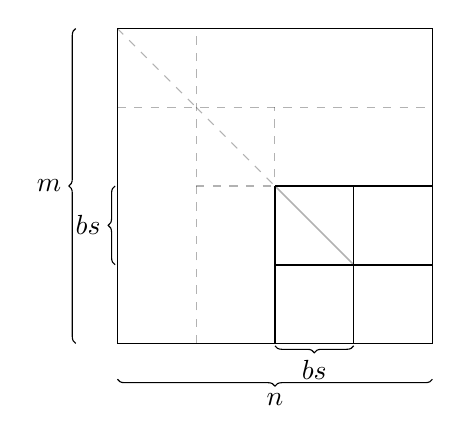
\begin{tikzpicture}
	\draw[semithick] (0,0) -- (4,0) -- (4,4) -- (0,4) -- (0,0);
	

		\draw[dashed,opacity=0.3] (1,0) -- (1,4);
		\draw[dashed,opacity=0.3] (0,3) -- (4,3);
		\draw[dashed,opacity=0.3] (0,4) -- (1,3);
		\draw[dashed,opacity=0.3] (2,0) -- (2,3);
		\draw[dashed,opacity=0.3] (1,2) -- (4,2);
		\draw[dashed,opacity=0.3] (1,3) -- (2,2);
		\draw[semithick,opacity=0.3] (2,2) -- (3,1);
		\draw[semithick] (2,1) -- (4,1);
		\draw[semithick] (3,2) -- (3,0);
		\draw[semithick] (2,2) -- (2,0);
		\draw[semithick] (2,2) -- (4,2);
		\draw[decorate, decoration={brace,mirror}, yshift=-.2ex]  (2,0) -- node[below=0.4ex] {$bs$}  (3,0);
		\draw[decorate, decoration={brace}, xshift=-.2ex]  (0,1) -- node[left=0.4ex] {$bs$}  (0,2);
	
	
	
	%\draw (0.5,3.5) node {$A_{0,0}$};
	%\draw (0.5,1.5) node {$A_{bs,0}$};
	%\draw (2.5,3.5) node {$A_{0,bs}$};
	%\draw (2.5,1.5) node {$A_{bs,bs}$};
	%\draw[decorate, decoration={brace,mirror}, yshift=-.2ex]  (0,0) -- node[below=0.4ex] {$bs$}  (1,0);
	%\draw[decorate, decoration={brace}, xshift=-.2ex]  (0,3) -- node[left=0.4ex] {$bs$}  (0,4);
	\draw[decorate, decoration={brace,mirror}, yshift=-3ex]  (0,0) -- node[below=0.4ex] {$n$}  (4,0);
	\draw[decorate, decoration={brace}, xshift=-3.5ex]  (0,0) -- node[left=0.4ex] {$m$}  (0,4);
	
	\end{tikzpicture}
\end{itemize}
\end{frame}

\clearpage
\setcounter{page}{8}
\begin{frame}
\frametitle{Geblockte QR-Zerlegung}
\begin{itemize}
	\item Matrix A\\
	\centering
	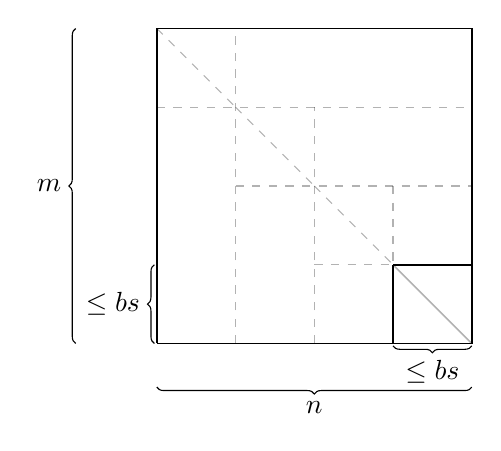
\begin{tikzpicture}
	\draw[semithick] (0,0) -- (4,0) -- (4,4) -- (0,4) -- (0,0);
	
		\draw[dashed,opacity=0.3] (1,0) -- (1,4);
		\draw[dashed,opacity=0.3] (0,3) -- (4,3);
		\draw[dashed,opacity=0.3] (0,4) -- (1,3);
		\draw[dashed,opacity=0.3] (2,0) -- (2,3);
		\draw[dashed,opacity=0.3] (1,2) -- (4,2);
		\draw[dashed,opacity=0.3] (1,3) -- (2,2);
		\draw[dashed,opacity=0.3] (2,2) -- (3,1);
		\draw[dashed,opacity=0.3] (2,1) -- (3,1);
		\draw[dashed,opacity=0.3] (3,2) -- (3,1);
		\draw[semithick] (3,1) -- (4,1);
		\draw[semithick] (3,1) -- (3,0);
		\draw[semithick,opacity=0.3] (3,1) -- (4,0);
		
	\draw[decorate, decoration={brace,mirror}, yshift=-.2ex]  (3,0) -- node[below=0.4ex] {$\le bs$}  (4,0);
	\draw[decorate, decoration={brace}, xshift=-.2ex]  (0,0) -- node[left=0.4ex] {$\le bs$}  (0,1);
	
	
	
	%\draw (0.5,3.5) node {$A_{0,0}$};
	%\draw (0.5,1.5) node {$A_{bs,0}$};
	%\draw (2.5,3.5) node {$A_{0,bs}$};
	%\draw (2.5,1.5) node {$A_{bs,bs}$};
	%\draw[decorate, decoration={brace,mirror}, yshift=-.2ex]  (0,0) -- node[below=0.4ex] {$bs$}  (1,0);
	%\draw[decorate, decoration={brace}, xshift=-.2ex]  (0,3) -- node[left=0.4ex] {$bs$}  (0,4);
	\draw[decorate, decoration={brace,mirror}, yshift=-3ex]  (0,-.1) -- node[below=0.4ex] {$n$}  (4,-.1);
	\draw[decorate, decoration={brace}, xshift=-3.5ex]  (-.5,0) -- node[left=0.4ex] {$m$}  (-.5,4);
	
	\end{tikzpicture}
\end{itemize}
\end{frame}

	\end{itemize}
\end{frame}

\begin{frame}
	\frametitle{Mehrere Householder-Transformationen anwenden}	
	\vspace{-1cm}	
		\begin{itemize}
			\item Ansatz\\
			\vspace{0.3cm}
			$\hat{H} = H_1H_2...H_k = I - VTV^T \quad \text{mit}\quad H_i = I - \tau_i v_iv_i^T $
			\vspace{0.3cm}
			\item Householder-Transformationen anwenden\\
			\vspace{0.3cm}
			$ C \leftarrow \hat{H} C = C - V T V^T C \quad $
			
		\end{itemize}

		\vspace{-3cm}
		\hspace{9.5cm}
		\centering
		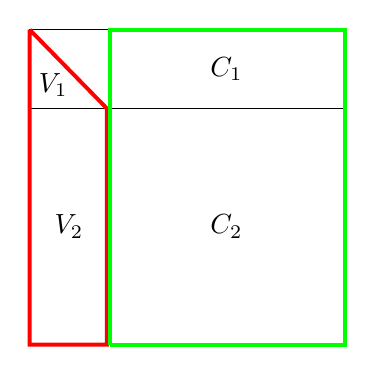
\begin{tikzpicture}
\draw[semithick] (0,0) -- (4,0) -- (4,4)-- (0,4)-- (0,0);

\draw[semithick] (1,0) -- (1,4);
\draw[semithick] (0,3) -- (4,3);
\draw[red, line width=0.5mm, opacity=1] (0,4) -- (0,0) -- (0.98,0) -- (0.98,3) -- (0,4);
\draw[green, line width=0.5mm, opacity=1] (1.02,0) -- (4,0) -- (4,4)-- (1.02,4)-- (1.02,0);


%\draw[decorate, decoration={brace,mirror}, yshift=-.5ex]  (0,0) -- node[below=0.4ex] {$k$}  (.95,0);
%\draw[decorate, decoration={brace}, xshift=-.5ex]  (0,3) -- node[left=0.2ex] {$k$}  (0,4);
%\draw[decorate, decoration={brace,mirror}, yshift=-.5ex]  (1.05,0) -- node[below=0.4ex] {$n$}  (4,0);
%\draw[decorate, decoration={brace}, xshift=-3ex]  (0,0) -- node[left=0.4ex] {$m$}  (0,4);

\draw (0.3,3.3) node {$V_1$};
\draw (0.5,1.5) node {$V_2$};
\draw (2.5,3.5) node {$C_1$};
\draw (2.5,1.5) node {$C_2$};

\end{tikzpicture}
\end{frame}



\begin{frame}
	\frametitle{Verschiedene Blockgrößen}
		\centering
	\scalebox{.85}{
		\includegraphics[width=\textwidth]{images/blkbs}
	}
\end{frame}

\begin{frame}
	\frametitle{Geblockte QR}
		\frametitle{Geblockte QR - Blocksizes}
	\centering
	\scalebox{.85}{
		\includegraphics[width=\textwidth]{images/both}
	}
\end{frame}




